\subsection*{Approach Overview}


\begin{figure}[t]
	\begin{center}
	  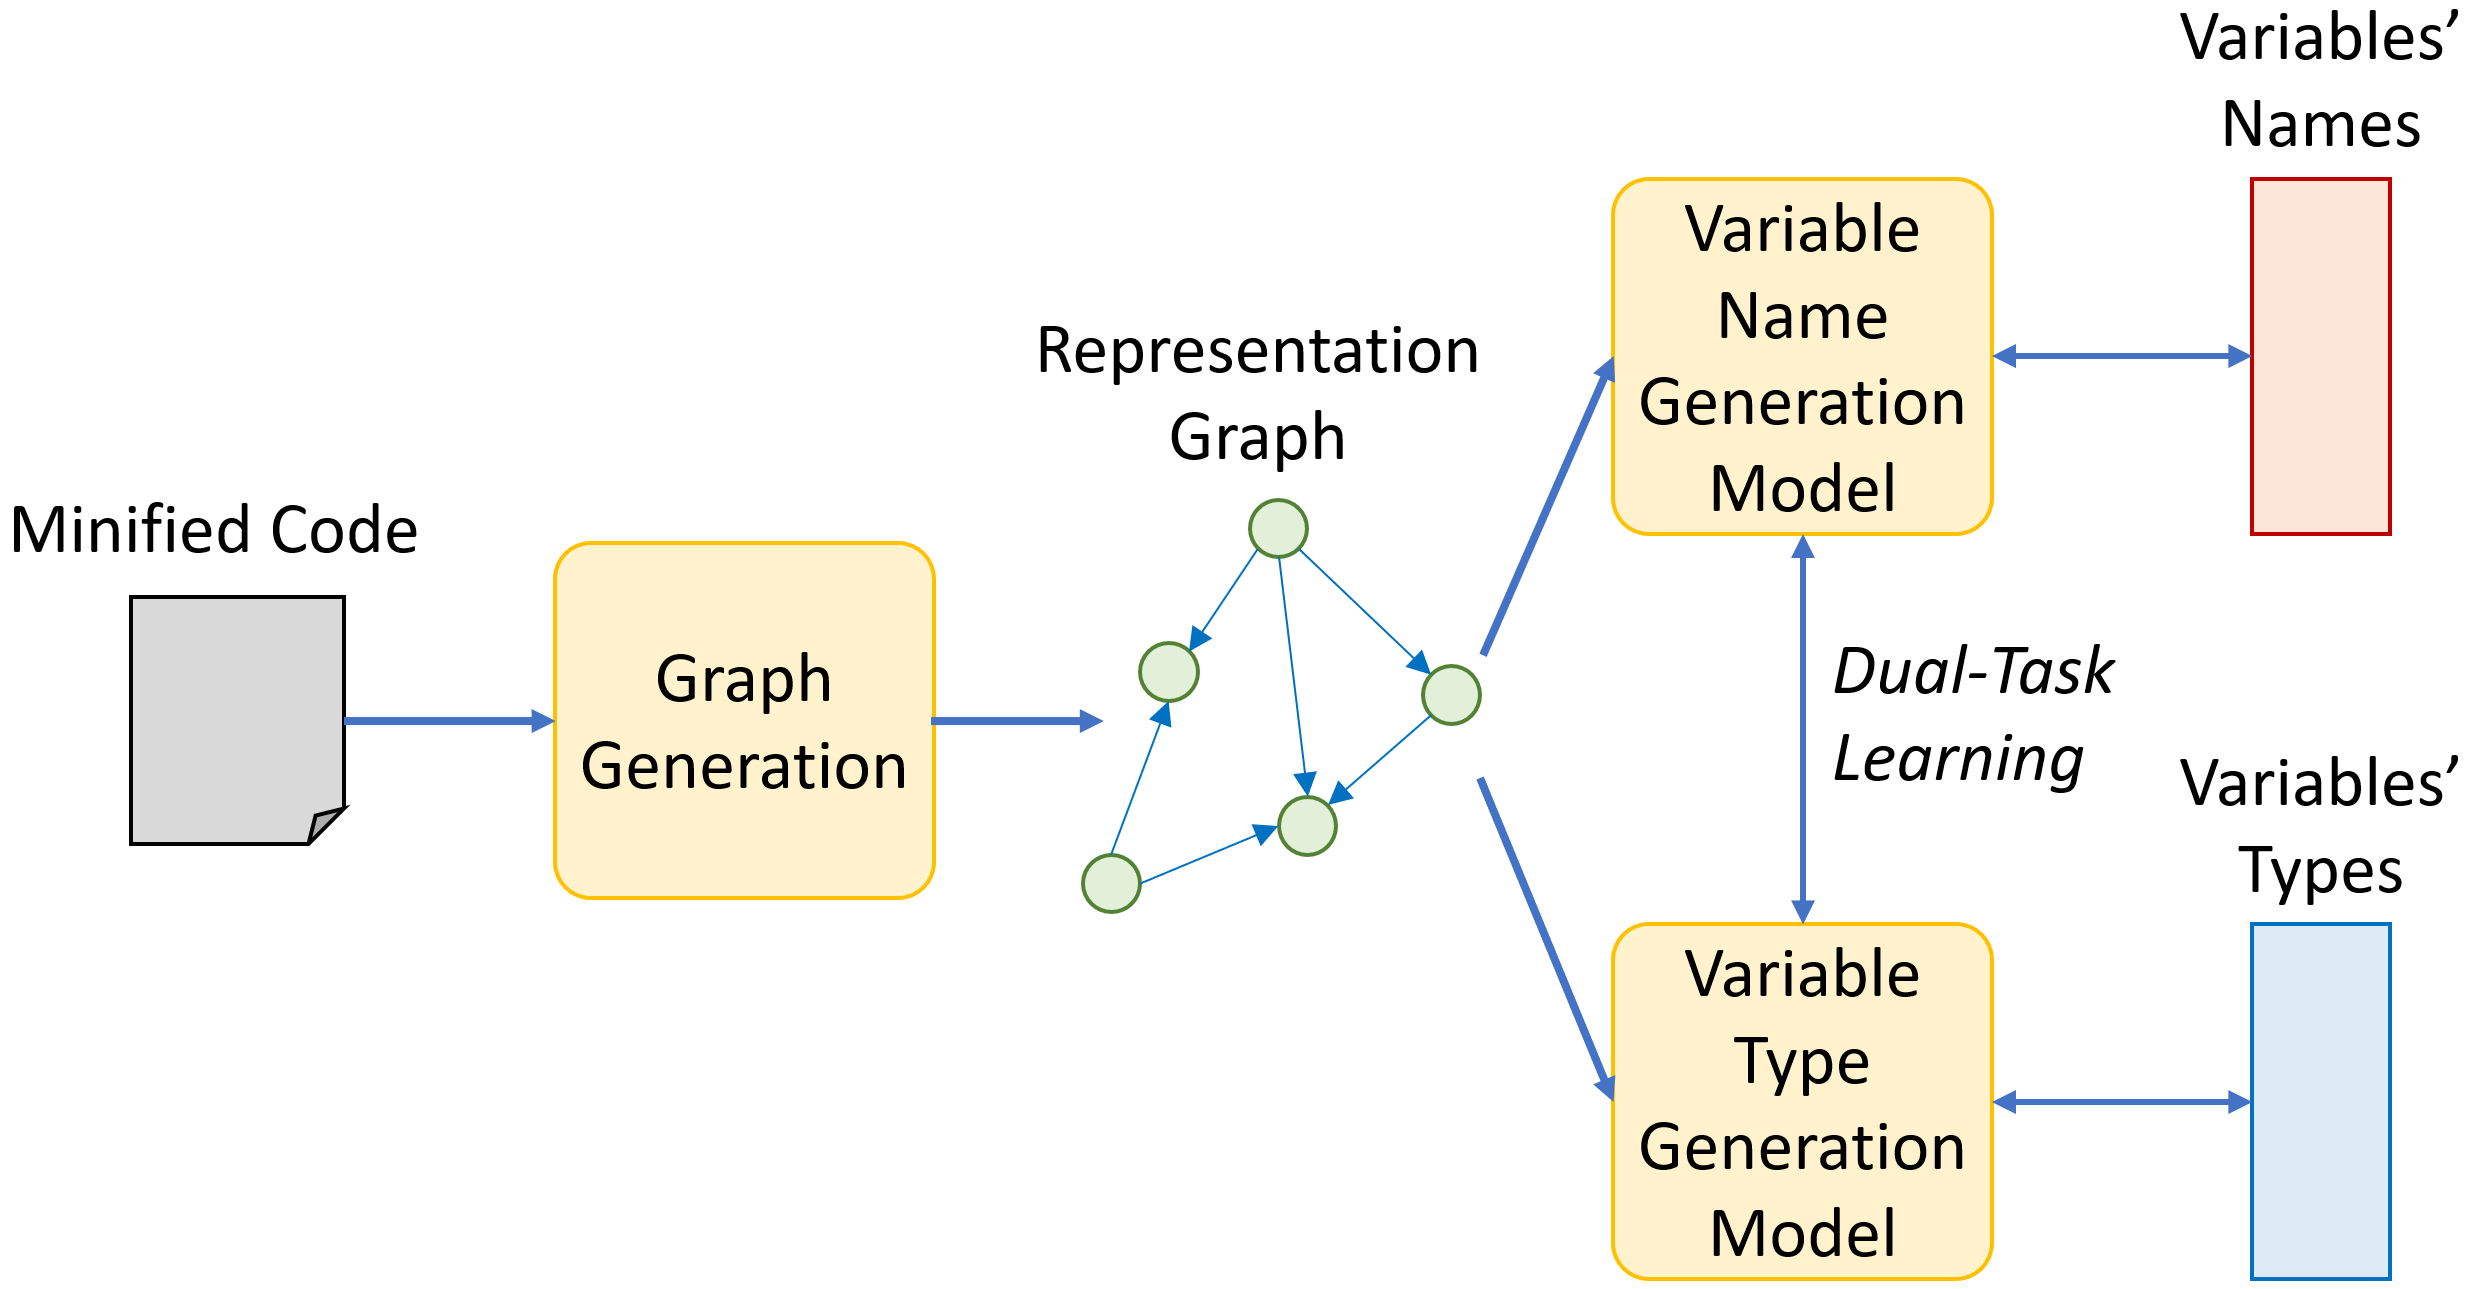
\includegraphics[width=3in]{figures/overview-2.png}
          \vspace{-10pt}
		\caption{{\tool}: Architecture Overview}
		\label{overview}
	\end{center}
\end{figure}

%\begin{figure}[t]
%	\begin{center}
%	  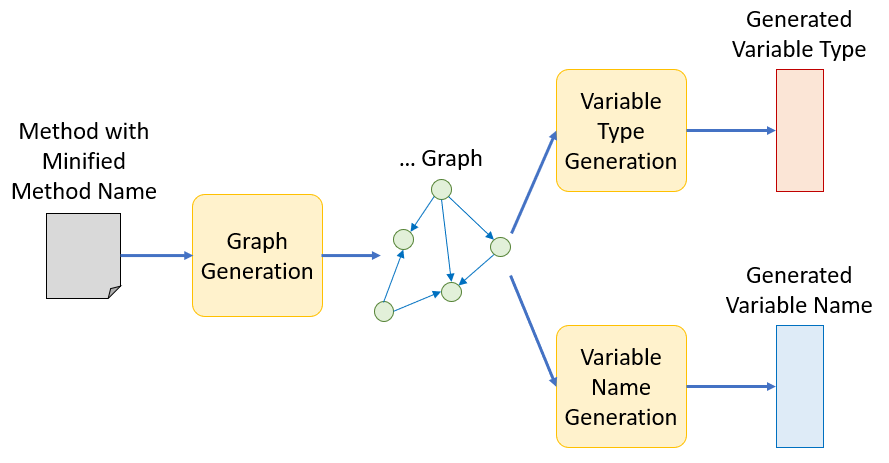
\includegraphics[width=\columnwidth]{figures/testing.png}
%          \vspace{-15pt}
%		\caption{Testing Process}
%		\label{predict_process}
%	\end{center}
%\end{figure}

%There are two main processes in {\tool}: training and predicting.

{\tool} accepts minified Python code and at the same time, recovers
the variable names and derives the types for variables/expressions. It
also can take regular Python code and derive the types.
%
Figure~\ref{overview} illustrates the overall process. The input is
the minified code with all the original variables' names and types
during training and without them during the prediction.
%
The process contains the following key steps. First, the minified code
is parsed and two feature graphs are extracted: 1) the Type Dependency
Graph~\cite{HiTyper-icse22} representing the relations among the
types of the variables in a function/method according to type
inference rules, and 2) the Relation Graph~\cite{icse19} represent the
relations among the variables including the ones via field accesses
and method calls (Section~\ref{sec:concepts}). The two graphs can
always be extracted for minified code in both training or
prediction. They will be merged into a representation graph.

We have two models dedicated to the two tasks: Variable Name
Generation (VNG) and Variable Type Generation (VTG). {\tool}
first extracts the features in a representation graph,
%(e.g., the variables' names, the names of the fields and methods),
and converts them into the input vectors for the VNG and VTG models.

The VNG model processes them as follows.
%extracts the features in the graph and builds the representation vectors.
For the nodes that represent the variables with the minified names, we
mask the node features and regard them as the missing features, and
then feed the graph into a Graph Convolutional
Network--Missing Features (GCNmf)~\cite{GCNmf}. The actual names of
the variables in the input minified code are used as the labels during
the training. For name prediction, the same
process is used except that the variables' names are predicted
by the trained VNG model. To generate names, we also use program
 rules to ensure scoping, and valid and consistent names.

The VTG model leverages Edge-Enhanced Graph Convolutional Networks
(EE-GCN)~\cite{ee-gcn} with the support of an embedding
model~\cite{pennington2014glove} as well as the Gate Recurrent Unit
(GRU). The actual variable types in the input minified code
are used as the labels during training. For prediction, the same
process is used except that the types are predicted
using the trained model. To generate the types, we use type
inference rules to eliminate the impossible candidates.

%To propagate the impact of type prediction to name prediction and vice
%versa,

To propagate the impact between VTG and VNG, we apply a dual-task
learning mechanism between them. We use the uncertainty weighted
multi-task loss as the loss function and use the
maximum of the top-1 accuracy scores from two tasks as the training
target.

To infer types for non-minified code, the representation graph is
extracted as explained, and then fed to {\tool} whose VTG will produce
the types for variables/expressions. The full variable names will help
VNG improve the type inference task by VTG.

%Step 1. Generate graphs...

%Step 2. Variable Type Generation:

%1> Graph edge represent different relations (This may change depends on the graph we finally want to use). Each node is a variable, method call, or a field of an object. We use the name of the variable (minified), method call, or the field as the node feature and use GloVe to learn the representation vector.

%2> We use EGCN that accepts graphs with both node features and edges features as input. Here the edge feature is the edge type.

%3> The output of EGCN is the generated representation vector $V_r$ for each node.

%4> We combined the representation vector we get from EGCN with the generated from the next step $V'_r$ (variable name generation) by using the cross-product and get the final generated representation vector for type prediction ($V_f$)

%5> We use a GRU (RNN) as decoder accepts the $V_f$ as input and generates the type for the variables as output.

%6> When generating the type, we use some basic rule from parser to reduce the possible candidates.

%Step 3. Variable Name Generation:

%1> Similar to step 2, we use GloVe to learn the representation vector.

%2> For the node that represent the variable with minified name, we mask the node feature and regard it as the missing feature.

%3> Put the graph with missing feature for some nodes into the $GCN_{mf}$ as input.

%4> The $GCN_{mf}$ can output the predicted missing node feature representation vector $V_{rm}$ and the node representation vector $V'_r$. The node representation vector $V'_r$ will be used in step 2.

%5> Use $V_{rm}$ as the input of a GRU (RNN) decoder, and the decoder generate the names for the variables with the minified name.

%6> When doing generation, we apply basic checking to make sure the same variable has only one consistent name.

%Step 4. Multi-task learning

%We use the uncertainty weighted multi-task loss as the multitask learning loss function and use the maximum of the top-1 accuracy score from two tasks as the training target.

